% Intestazione
\fancyhead[L]{3 \hspace{0.2cm} Processi di Supporto} % Testo a sinistra


\section{Processi di Supporto}

\subsection{Documentazione}
\label{sec:documentazione}

\subsubsection{Scopo}
Il \emph{processo}\textsubscript{\textit{\textbf{G}}} di documentazione mira a raccogliere le informazioni prodotte da un processo o
da un’attività nel \emph{ciclo di vita}\textsubscript{\textit{\textbf{G}}}, le decisioni prese dal gruppo e gli standard adottati per lo
svolgimento del progetto. È obbligatorio per tutti i membri del gruppo il rispetto di queste regole.

\subsubsection{Descrizione}
La documentazione costituisce una componente essenziale del progetto, poichè consente di
registrare ogni aspetto del lavoro svolto e delle decisioni prese. In particolare, questa sezione
raccoglie tutte le norme relative alla creazione, all’aggiornamento e al mantenimento della
documentazione (interna ed esterna) prodotta dal gruppo \emph{SWEg Labs} per ciascuna fase del
ciclo di vita del software.

\subsubsection{Aspettative}
Per quanto riguarda il processo di documentazione, il team ha le seguenti aspettative:
\begin{itemize}
    \item Definire delle procedure ripetibili che permettano di standardizzare il \emph{way of working}\textsubscript{\textit{\textbf{G}}}
    e la documentazione prodotta dal gruppo;
    \item Dichiarare le norme che i membri del gruppo sono tenuti a seguire per semplificare la
    redazione dei documenti.
\end{itemize}

\subsubsection{Ciclo di vita dei documenti}
Il ciclo di vita di ogni documento si compone delle seguenti fasi, visibili in Figura \bulref{fig:ciclo_vita_documentazione}:
\begin{itemize}
    \item \textbf{Redazione}:  documenti vengono scritti seguendo un approccio incrementale, e sono
    considerati redatti soltanto una volta completata la loro stesura;
    \item \textbf{Verifica}\textsubscript{\textit{\textbf{G}}}: ogni volta che i documenti vengono modificati necessitano di una verifica. 
    Ogni sezione coinvolta nella modifica di un documento viene verificata da una
    o più persone, chiamate verificatori. Il documento è considerato verificato una volta
    completate le verifiche da parte di tutti i verificatori incaricati;
    \item \textbf{Approvazione}: in questa fase, il Responsabile di Progetto dichiara che il documento
    è pronto per essere rilasciato, cioè che la sua stesura è completata ed è stato verificato.
    A questo punto, il documento viene marcato come approvato.
\end{itemize}

\begin{figure}[h]
    \centering
    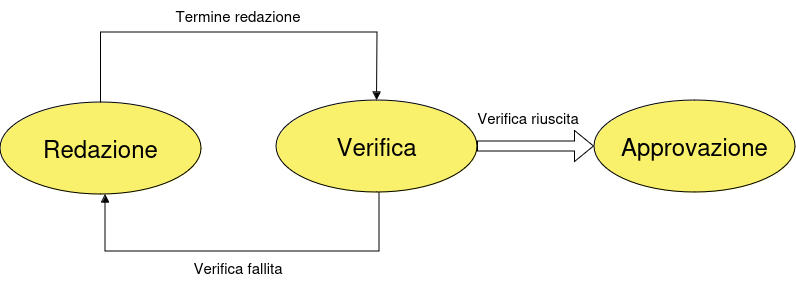
\includegraphics[width=0.6\textwidth]{Ciclo di vita della documentazione.png}
    \caption{Ciclo di vita della documentazione}
    \label{fig:ciclo_vita_documentazione}
\end{figure}

\subsubsection{Struttura dei documenti}
Ogni documento che verrà prodotto dovrà seguire una precisa struttura per garantire 
omogeneità e coesione.

\subsubsubsection{Numerazione di pagine}
La numerazione delle pagine del documento segue uno schema ben definito. Dalle pagine
iniziali e fino alla pagina precedente l’inizio del primo capitolo, viene utilizzata la numerazione
romana. Questa scelta mira a differenziare chiaramente la sezione introduttiva dal resto
del testo principale. Dopo questa fase preliminare, la numerazione prosegue con numeri
arabi, partendo da 1. Questo sistema offre una chiara progressione nel corpo principale del
lavoro. \\
Nel caso di appendici, la numerazione ritorna all’uso dei numeri romani, assegnando il numero 
I a ciascuna appendice.  Se ci sono più appendici, ogni volta che ne viene completata
una, si ricomincia la numerazione da I per la successiva. Questo approccio fornisce
un’organizzazione chiara e logica per le appendici, garantendo che ciascuna sia distintamente 
identificata. L’uso coerente di numeri romani e arabi in diverse sezioni del documento
contribuisce a una struttura ordinata e comprensibile per il lettore.

\subsubsubsection{Intestazione e piè di pagina}
In ciascuna pagina del documento, escludendo il frontespizio, sono presenti sia un’intestazione
che un piè di pagina. Nell’intestazione, sono inclusi i seguenti elementi:
\begin{itemize}
    \item Sul lato sinistro: il numero e il titolo del capitolo corrente;
    \item Sul lato destro: il logo del gruppo.
\end{itemize}
Nel piè di pagina, invece, sono indicati i seguenti dettagli:
\begin{itemize}
    \item Sul lato sinistro: il nome del file;
    \item Al centro: il numero della pagina attualmente in consultazione;
    \item Sul lato destro: il numero di versione del file.
\end{itemize}

\subsubsubsection{Frontespizio}
Il frontespizio, ovvero la prima pagina del documento,  strutturato nel seguente modo:
\begin{itemize}
    \item \textbf{Logo UniPD}: il logo universitario è posizionato in alto a sinistra;
    \item \textbf{Informazioni sul corso}: le informazioni relative al corso di Ingegneria del Software sono in alto a destra
    \item \textbf{Logo del gruppo}: il logo del gruppo è posizionato in alto a sinistra subito sotto al logo dell'Università;
    \item \textbf{Nome gruppo e recapito}: le informazioni sul gruppo \emph{SWEg Labs} sono posizionate in alto a destra, subito sotto alle info sul corso;
    \item \textbf{Titolo}: il titolo del documento è posizionato al centro della pagina, in grassetto;
    \item \textbf{Versione}: la versione del documento è posizionata al centro della pagina, appena sotto il titolo;
    \item \textbf{Tabella descrittiva}: posizionata centralmente sotto la versione del documento, riporta le seguenti informazioni:
    \begin{itemize}
        \item \textbf{Stato}: lo stato del documento nel suo ciclo di vita;
        \item \textbf{Redazione}: elenco dei membri del gruppo (nome e cognome) che hanno svolto la redazione del documento;
        \item \textbf{Verifica}: elenco dei membri del gruppo (nome e cognome) che hanno svolto la verifica del documento;
        \item \textbf{Approvazione}: elenco dei membri del gruppo (nome e cognome) che hanno svolto l’approvazione del documento;
        \item \textbf{Proprietario}: il proprietario del documento, nel nostro caso tutto il gruppo \emph{SWEg Labs};
        \item \textbf{Uso}: destinazione d’uso del documento (interno o esterno);
        \item \textbf{Destinatari}: destinatari del documento.
    \end{itemize}
\end{itemize}